\documentclass[a4paper, 10pt]{article}

\usepackage[margin = 1in]{geometry} % for spacing around
\usepackage{graphicx} % for including images in your pdfs
\usepackage{xcolor} % for including colors in your pdf
\usepackage{soul} % for text decoration
\usepackage[utf8]{inputenc} % for encoded text
\usepackage[T1]{fontenc}
\usepackage{setspace} % for setting different line spacings between paragrafs.
\usepackage{enumerate} % for letting us get more detailed enumerate lists
\usepackage{multirow} % to let us combine more rows together
\usepackage{colortbl} % for decorating tables
\usepackage{amsmath} % used for representing more complicated math displays
\usepackage{supertabular}
\usepackage{longtable} % both of these packages are used to making really big tables
\usepackage{wrapfig} % allows us to wrap text around figures
\usepackage{fancyhdr} % for making fancy headers
%\usepackage{bibtex} % for making better bibliographies
\usepackage[pdftex]{hyperref} % for letting us make links
\usepackage{lscape} % Allows us to flip from portrait to landspace
\usepackage{tikz} % for high detailed drawing
\usepackage{multicol} % To put things side by side
\usepackage{rotating} % For rotating objects
% \usepackage{draftwatermark} % For adding watermarks
\usepackage{MnSymbol} % for using multiple symbols
\usepackage{mathtools} % Used for more math symbols
\usepackage{xfrac} % For more complciated fractions and to add derivitives
\usepackage{enumitem} % for better enum lists
\usepackage{tcolorbox} % for adding colored text boxes
\usepackage{bm} % Adding bold text to math inputs
\usepackage{pgfplots} % Used for plotting functions
\usepackage{wallpaper} % For adding wallpapers
\usepackage{listings} % Required for insertion of code
\usepackage{eso-pic} % Required for placing background pictures
\usepackage{ifthen} % Required for conditional statements
\usepackage[backend=biber, style=alphabetic, citestyle=authoryear]{biblatex}

% Define the Haskell language style for listings
\lstdefinelanguage{Haskell}{
    morekeywords={class, data, deriving, do, else, if, import, in, infixl, infixr, instance, let, module, newtype, of, then, type, where, _, ::, =, \, |, <-, ->, @, ~, =>},
    sensitive=true,
    morecomment=[l]{--},
    morecomment=[s]{\{-}{-\}},
    morestring=[b]",
    stringstyle=\color{red},
    identifierstyle=\color{blue},
    keywordstyle=\color{green},
    commentstyle=\color{gray},
    basicstyle=\ttfamily, % Use monospaced font for code
    showstringspaces=false, % Don't show spaces in strings as special underscores
    numbers=left, % Line numbers on the left
    numberstyle=\tiny\color{gray}, % Line numbers are grey and small
    stepnumber=1 % Line numbers go in steps of 1
}

\lstset{
    backgroundcolor=\color{gray!10},  % set backgroundcolor
    basicstyle=\footnotesize\ttfamily, % set font and size
    breaklines=true,                   % automatic line breaking
    captionpos=b,                      % caption-position - bottom
    frame=single,                      % adds a frame around the code
    rulecolor=\color{black},           % if not set, the frame-color may be changed on line-breaks within not-black text
}

% Setting up the default image path
\graphicspath{{./Images/}}

% Add the bib file with all references
\addbibresource{./references.bib}

% Implementing authro details
\title{Introduction to Haskell Programming Language}
\author{Emre Arapcic-Uevak}
\date{}

% Setting up the fancy page style
\fancypagestyle{customStyle}{
	\lhead{} \chead{} \rhead{}
	\lfoot{} \cfoot{\thepage} \rfoot{}
	\renewcommand{\headrulewidth}{0pt}
	\renewcommand{\footrulewidth}{1pt}
}
\pagestyle{customStyle}

% Setting up hyperref options
\hypersetup {
	colorlinks = false,
	citecolor = black,
	filecolor = blue,
	linkcolor = blue,
	urlcolor = blue,
	pdftex
}

% Custom commands


\begin{document}
	\maketitle
    \lstset{language=Haskell}
	\vspace{5mm}
	
	\begin{abstract}
		\begin{center}
            \begin{spacing}{1.0}
                This presentation introduces the Haskell programming language, covering its history, key features, data structures, comparisons with other languages, and providing simple code examples. The audience will gain insights into the fundamentals of Haskell and its applications in modern programming.
            \end{spacing}
		\end{center}
	\end{abstract}

	\ThisCenterWallPaper{.4}{Images/IUS Logo.png}

	\newpage % Start new page after the first page
    \AddToShipoutPictureBG{%
        \ifthenelse{\value{page}=1}{}{%
            \begin{tikzpicture}[remember picture,overlay]
                \node [opacity=0.3, at=(current page.center)] {
                    
\includegraphics[width=0.5\paperwidth]{Haskell-Logo}
                };
            \end{tikzpicture}
        }
    }

	\tableofcontents
	\pagebreak

    \setstretch{1.5}  % 1.5 line spacing for the entire document

	\section{Introduction to Haskell}
        \noindent Haskell is a purely functional programming language, distinguished by its strong static typing, high level of abstraction, and lazy evaluation. Inspired by the principles of lambda calculus, Haskell emphasizes functions without side effects and immutable data. Named after the logician Haskell Curry, it stands apart from imperative programming languages by treating computation as the evaluation of mathematical functions, thereby avoiding changing-state and mutable data.
	\section{History and Evolution of Haskell}
        \subsection{The Foundational Principles}
            Haskell's journey begins with its roots deeply embedded in lambda calculus, a sophisticated mathematical system devised by Alonzo Church in 1932. This system, focusing on function abstraction and application, forms the core of Haskell's functional programming ethos.

        \subsection{The Dawn of Functional Programming}
            Tracing its lineage to the 1960s, Haskell shares its heritage with LISP, the first functional language, born in 1959. However, Haskell emerged as a response to the limitations of its predecessors like ML, Hope, and Miranda, which, despite their innovations, struggled in practical application and widespread adoption.

        \subsection{The Formation of Haskell}
            Haskell's story officially starts at the FPCA '87 conference in Portland, Oregon. Here, a visionary group of academics united to forge a new path in programming language design. Their collaboration led to the first Haskell report in 1990, laying out the motivations, aspirations, and the unique nature of Haskell.

        \subsection{Milestones in Haskell’s Journey}
            Haskell's evolution saw pivotal moments, such as the release of the "Gentle Introduction to Haskell" tutorial and the advent of its essential tools – the GHC compiler and GHCI interpreter in 1992. At a seminal meeting at Yale in 1988, Haskell's goals were crystallized, focusing on research, teaching, and the development of robust systems.

        \subsection{A Tribute to Haskell B. Curry}
            Named to honor the eminent logician and mathematician Haskell B. Curry, the language reflects his groundbreaking work. Successive versions, including the Haskell Report 1.1 and version 1.2, introduced nuanced enhancements, shaping Haskell into the language we recognize today.

        \subsection{Haskell in the Digital Age}
            Marking its online presence, Haskell took to the internet in 1994 with haskell.org, a domain that continues to be a hub for enthusiasts. The release of Haskell version 1.3 in 1996 was a landmark, introducing significant refinements and capabilities.

        \subsection{Haskell 98 - A Commitment to Stability}
            The publication of "The Haskell 98 Report: Language and Libraries" in 1999 was a declaration of Haskell's maturity and stability, broadening its appeal and application. This version, later available freely online, cemented Haskell's place in the programming world.

        \subsection{The 21st Century and Haskell Prime}
            With the turn of the century, Haskell faced the need for evolution. The emergence of Haskell Prime (Haskell$'$) signified a modernized, incrementally developed version, with Haskell 2010 being its first notable iteration.

        \subsection{Haskell Today}
            Haskell's narrative continues to unfold, with the Haskell Foundation, established in 2020, championing its development. The support from numerous companies ensures Haskell's enduring presence and evolution in the realm of functional programming.

    \pagebreak
	\section{Features of the Language}
        Haskell is distinguished by a range of unique and powerful features, each contributing to its robustness as a functional programming language.

        \subsection{Purely Functional Programming}
            Haskell is a purely functional language, ensuring functions are free from side effects. This approach simplifies both debugging and testing, as the same input always yields the same output.

        \subsection{Strong, Static Type System with Type Inference}
            The language boasts a robust and static type system, with type checking at compile time to minimize runtime errors. Type inference in Haskell allows for less verbose code while maintaining type safety.

        \subsection{Lazy Evaluation}
            Haskell employs lazy evaluation, delaying computations until their results are needed. This leads to efficient memory utilization and the ability to define infinite data structures.

        \subsection{Immutability}
            Variables in Haskell are immutable. Once a value is assigned to a variable, it cannot be altered, which aids in reducing side effects and simplifying code maintenance.

        \subsection{First-Class Functions}
            Functions in Haskell are treated as first-class citizens, capable of being passed as arguments, returned from other functions, and assigned to variables.

        \subsection{Pattern Matching}
            Haskell offers advanced pattern matching capabilities, allowing for concise and readable code through the direct decomposition of data structures.

        \subsection{High-Level Abstractions}
            The language supports high-level abstractions such as monads, facilitating the management of complex computational patterns like side effects.

        \subsection{Concurrent and Parallel Programming}
            Haskell excels in concurrent and parallel programming, streamlining the development of efficient multi-core processor applications.

        \subsection{Extensive Standard Library}
            Haskell is equipped with a comprehensive standard library, covering a broad spectrum of functionalities, from basic data manipulation to sophisticated algorithms.

        \pagebreak

	\section{Structures of the Language}
        Haskell's design and architecture are characterized by several key structural elements, which make it unique and powerful among programming languages.

        \subsection{Syntax and Notation}
            Haskell features a clean and concise syntax that emphasizes readability and maintainability. It uses significant whitespace and layout rules, similar to Python, to define code structure, reducing the reliance on braces and semicolons.
            \textbf{Key Aspects of Haskell's Syntax:}
            \begin{itemize}
                \item \textit{Function Definition and Application:} Functions are defined using a straightforward syntax, where the function name is followed by its parameters, and the body of the function follows an equals sign. Function application is equally straightforward, requiring only the function name followed by its arguments, without parentheses or commas.
                \item \textit{Indentation-Sensitive:} Haskell's layout rule dictates that code grouped together (like the body of a function or a control structure) must be indented under the same column. This leads to a visually structured and clean code layout.
                \item \textit{Infix and Prefix Notation:} Haskell allows both infix and prefix notation for functions, enhancing flexibility and readability in different contexts. For example, operators like `+` are used infix, while most other functions are used in prefix form.
            \end{itemize}

            \textbf{Example of Haskell Syntax:}
            Consider a simple function definition in Haskell:

            \begin{lstlisting}
addNumbers :: Int -> Int -> Int
addNumbers x y = x + y
            \end{lstlisting}

            This function `addNumbers` takes two integers (`Int`) as inputs and returns their sum. The type declaration (`::`) is optional but helps in understanding the function's contract. Notice the absence of curly braces and semicolons, and how the function's body is simply defined after the equals sign.

            Haskell's syntax, while different from many mainstream languages, offers a level of expressiveness and clarity that is appreciated in complex software development.

        \newpage
        \subsection{Basic Types}

            Haskell's standard library includes several built-in basic types that are fundamental to the language. The most commonly used are:

            \begin{itemize}
                \item \texttt{Bool} for boolean values.
                \item \texttt{Char} for single Unicode characters.
                \item \texttt{String}, which is syntactically equivalent to a list of characters (\texttt{[Char]}).
                \item \texttt{Int} for fixed-precision integers, typically 64 bits in size on modern systems.
                \item \texttt{Integer} for arbitrary-precision integers, limited only by available memory.
                \item \texttt{Float} for single-precision floating-point numbers.
                \item \texttt{Double} for double-precision floating-point numbers.
            \end{itemize}

            \noindent It's worth noting that numeric literals in Haskell are polymorphic. They can represent any numeric type based on the context in which they are used.

            \noindent Here are some illustrative examples:

            \begin{lstlisting}
x :: Int
x = 42  -- Represents a fixed-size integer

y :: Double
y = 3.14  -- Represents a double-precision floating-point number

isTrue :: Bool
isTrue = true  -- Represents a boolean value

charExample :: Char
charExample = 'A'  -- Represents a single character

bigInt :: Integer
bigInt = 123456789012345678901234567890  -- Represents an arbitrary-size integer

someString :: String
someString = "This is a string"  -- Represents a string, equivalent to a list of characters
            \end{lstlisting}

        \newpage
        \subsection{Explicit and Implicit Declaration (Type Inferencing)}
            \noindent Haskell allows for both explicit and implicit type declarations. Explicit declaration is specifying the type of a variable or function using the double colon operator \texttt{::}, while implicit declaration leverages the compiler's type inference system.

            \begin{lstlisting}
myVar :: String
myVar = "CS305"
            \end{lstlisting}

            Implicit type declaration does not require specifying types, as the compiler deduces the type from the values used.

            \begin{lstlisting}
myVar = "CS305"  -- The compiler infers myVar as a String
            \end{lstlisting}

        \subsection{Comments}
            Comments are integral to writing clear and maintainable code. In Haskell, as in many programming languages, comments come in two forms: single-line and multi-line. Single-line comments are denoted by \texttt{--} and extend to the end of the line. Multi-line comments are enclosed within \texttt{\{-} and \texttt{-\}}, and uniquely, they can be nested within one another, which is a feature not commonly found in all programming languages.

            \lstset{language=Haskell}
            \begin{lstlisting}
-- This is a single-line comment

{-
This
is
a
multi-line
comment
which can be {- nested -} within another comment
-}
            \end{lstlisting}

            These commenting conventions facilitate the documentation of code and the temporary disabling of code blocks during debugging and development.

        \newpage
        \subsection{Immutability}

            Immutability is a cornerstone of Haskell's design, mandating that variables, once assigned, cannot be altered. This principle underpins the functional programming paradigm, where data stability and predictability are paramount.

            \lstset{language=Haskell}
            \begin{lstlisting}
someVar :: String
someVar = "Modify me"

-- Reassignment is not allowed and results in a compile-time error:
-- someVar = "modified"  -- This causes a multiple declaration error
            \end{lstlisting}

            \noindent Attempting to reassign `someVar` to a new value here would result in a compile-time error, specifically a "multiple declaration error," indicating that `someVar` has been assigned a value more than once.
            
            \vspace{5mm}
            \noindent This approach contrasts with mutable languages, where variables can change state throughout their lifecycle. While immutability can lead to a more functional and safer codebase, it may require programmers to think differently, particularly when it comes to managing state and side effects. Some of the benefits include easier reasoning about code behavior and enhanced thread safety. However, it may also introduce overhead due to the creation of new instances and could necessitate a deeper understanding of recursion and state management techniques within Haskell's functional context.


    \subsection{Lists}
        A list in Haskell is a collection of elements of the same type, enclosed in square brackets and separated by commas. Haskell lists are zero-indexed and can be manipulated using a variety of functions, such as \texttt{head} for the first element, \texttt{tail} for all but the first element, and \texttt{length} for the number of elements.

        \lstset{language=Haskell}
        \begin{lstlisting}
nums :: [Int] -- This type declaration is optional
nums = [1, 2, 3, 4, 5]
        \end{lstlisting}

        \noindent Haskell's lazy evaluation model allows for lists to be potentially infinite. This feature enables defining lists without predetermined bounds, such as the list of all positive integers:

        \begin{lstlisting}
positiveIntegers = [1..] -- An infinite list of positive integers
        \end{lstlisting}

        \noindent Lazy evaluation ensures that operations on such infinite lists are still manageable, as elements are only computed as needed. For instance, list comprehensions can be used to create lists from existing lists:

        \begin{lstlisting}
squares = [x * x | x <- [1..10]] -- List of squares from 1 to 10
        \end{lstlisting}

        \noindent This list comprehension takes numbers 1 through 10 and returns a new list of their squares. Operations like these demonstrate the power and flexibility of Haskell's list handling capabilities.

        \newpage

        \subsection{Tuples}

            In Haskell, a tuple is a collection of finite, ordered elements that can be of different types. Tuples are particularly useful for grouping together a fixed number of items because they can hold multiple values together as a single unit.

            \begin{lstlisting}
-- A pair (2-tuple) consisting of a String and an Int
personInfo :: (String, Int)
personInfo = ("Alice", 42)

-- A triple (3-tuple) with different types
mixedTuple :: (String, Int, Bool)
mixedTuple = ("Bob", 28, True)

-- The empty tuple (0-tuple), which can be useful as a placeholder
emptyTuple :: ()
emptyTuple = ()
            \end{lstlisting}

            \noindent Each value in a tuple can be accessed through pattern matching, which allows for concise and expressive unpacking of the tuple's elements.

            \begin{lstlisting}
-- Pattern matching to extract values from a tuple
(name, age) = personInfo
            \end{lstlisting}

            \noindent This pattern matching expression binds `name` to `"Alice"` and `age` to `42`, extracting the elements of the `personInfo` tuple. Unlike lists, tuples are heterogenous, meaning each element can be of a different type, and their size is fixed upon creation. They are commonly used to return multiple values from a function and are an essential data structure in Haskell's type system.

        \newpage
        \subsection{Standard Prelude}

            The Haskell standard library, or standard prelude, includes a collection of built-in functions that are automatically imported into every Haskell program. These functions encompass a wide array of operations, including but not limited to, those that manipulate lists.

            \lstset{language=Haskell}
            \begin{lstlisting}
-- Selecting the first element of a non-empty list will return the element,
-- but using 'head' on an empty list will result in a runtime error.
res1 = head [1, 2, 3, 4, 5] -- 1

-- Similarly, 'tail' will fail on an empty list.
res2 = tail [1, 2, 3, 4, 5] -- [2, 3, 4, 5]

-- Indexing is zero-based, which means '!! 2' returns the third element.
res3 = [1, 2, 3, 4, 5] !! 2 -- 3

-- The 'take' function is efficient, but 'drop' might require traversing the list.
res4 = take 3 [1, 2, 3, 4, 5] -- [1, 2, 3]
res5 = drop 4 [1, 2, 3, 4, 5] -- [5]

-- 'length' and 'reverse' require traversing the entire list, leading to linear time complexity.
res6 = length [1, 2, 3, 4, 5] -- 5
res11 = reverse [1, 2, 3, 4, 5] -- [5, 4, 3, 2, 1]

-- List concatenation with '++' and constructing lists with ':' are commonly used operations.
res9 = [1, 2] ++ [3] ++ [4, 5] -- [1,2,3,4,5]
res10 = 0 : [1, 2, 3, 4, 5] -- [0, 1, 2, 3, 4, 5]

-- Reductions like 'sum' and 'product' can be implemented using 'foldl' or 'foldr'.
res7 = sum [1, 2, 3, 4, 5] -- 15
res8 = product [1, 2, 3, 4, 5] -- 120
res12 = foldl (+) 0 [1, 2, 3, 4, 5] -- Also 15
            \end{lstlisting}

            \noindent These examples illustrate the versatility of list processing in Haskell. The language's rich set of list operations enables programmers to write concise, clear, and expressive code.

            \newpage

    \subsection{Functions}

        In Haskell, a function is a mapping from arguments of one type to results of another type. The notation \texttt{T1 -> T2} denotes functions that map arguments of type \texttt{T1} to results of type \texttt{T2}.

        \lstset{language=Haskell}
        \begin{lstlisting}
-- A function to calculate the sum of two integers
-- (parameter, parameter) -> return
add :: (Int, Int) -> Int -- Function type declaration is optional
add (x, y) = x + y       -- Function definition is required

res1 = add (3, 2)        -- Evaluates to 5

-- Another way to define a function is by using currying,
-- where each argument is passed separately.
-- parameter -> parameter -> return
add2 :: Int -> Int -> Int -- Type declaration is optional
add2 x y = x + y

res2 = add2 3 2           -- Also evaluates to 5
        \end{lstlisting}

        \noindent The function \texttt{add} takes a single parameter: a tuple of two integers. In contrast, \texttt{add2} showcases currying, where a function takes its arguments one at a time. Currying enables partial application, where a function can be applied to some of its arguments to produce another function. For example:

        \begin{lstlisting}
addThree :: Int -> Int
addThree = add2 3

res3 = addThree 2         -- Evaluates to 5
        \end{lstlisting}

        \noindent The partially applied function \texttt{addThree} is created by supplying only the first argument to \texttt{add2}. This new function can then be used to add three to another number, demonstrating Haskell's elegant approach to function composition and application.
        \newpage

        \subsection{Function Composition}
            Function composition in Haskell is a way to combine two or more functions into a single function. The composition operator \texttt{(.)} is used to achieve this, where \texttt{(f . g)} is equivalent to \texttt{(\textbackslash x $\rightarrow$ f (g x))} in Haskell. This means that the result of applying function \texttt{g} to some input \texttt{x} is then passed as the argument to function \texttt{f}.

            \lstset{language=Haskell}
            \begin{lstlisting}
-- Type declaration of the composition operator
(.) :: (b -> c) -> (a -> b) -> a -> c

-- Example of composing two functions
(f . g) -- This is equivalent to the lambda expression below
(\x -> f (g x))
            \end{lstlisting}

            \noindent Function composition is a powerful concept in functional programming because it allows for the creation of complex operations by combining simpler ones. The composition operator is central to this idea, enabling concise and expressive function chaining.


        \subsection{Anonymous Functions}

            Anonymous functions, or lambda functions, are functions that are not bound to an identifier. In Haskell, anonymous functions are defined using a backslash (\textbackslash) followed by a list of parameters, an arrow (\texttt{->}), and then the function body. They are useful for creating quick, one-off functions without the need to give them a name.

            \lstset{language=Haskell}
            \begin{lstlisting}
-- An example of an anonymous function that adds two numbers
(\x y -> x + y)

-- Using an anonymous function with the map function
map (\x -> x * 2) [1, 2, 3, 4, 5] -- [2, 4, 6, 8, 10]
            \end{lstlisting}

            \noindent Anonymous functions are often used in higher-order functions, like \texttt{map}, \texttt{filter}, and \texttt{foldr}, where you need to pass a function as an argument. Since Haskell supports first-class functions, you can use anonymous functions wherever a function is expected.
            \newpage

     \subsection{Higher-Order Functions}
            In Haskell, it is possible to define functions that accept other functions as arguments, which classifies them as higher-order functions. A classic example of this is the \texttt{map} function, which applies a given function to each item in a list.
            Here's a simple example:

            \begin{lstlisting}
squareNum :: Int -> Int
squareNum n = n * n

nums :: [Int]
nums = [1, 2, 3, 4, 5]

res = map squareNum nums -- [1, 4, 9, 16, 25]
            \end{lstlisting}

            \noindent The function \texttt{squareNum} squares an integer. The list \texttt{nums} contains several integers. The \texttt{map} function is then used to apply \texttt{squareNum} to every element in \texttt{nums}, resulting in a new list \texttt{res} with each number squared.


        \newpage
        \subsection{Conditional Expressions}
            Haskell enables the use of conditional expressions for selecting between different results based on a given condition. The most fundamental form is the `if-then-else` expression, which must always end with an `else` branch to ensure that the expression is well-defined in all cases.

            \lstset{language=Haskell}
            \begin{lstlisting}
-- A function to calculate the absolute value of an integer
getAbs :: Int -> Int
getAbs x = if (x < 0) then -x else x

-- Example usage of getAbs
res1 = getAbs (-5) -- 5
res2 = getAbs 20   -- 20

-- Conditional expressions can be nested to handle multiple conditions
getSomething :: Int -> String
getSomething x = if (x < 0) then "Num is less than zero"
             else if (x > 0) then "Num is greater than zero"
             else "Num is zero"

-- Example usage of getSomething
res1 = getSomething (-5) -- "Num is less than zero"
res2 = getSomething 20   -- "Num is greater than zero"
res3 = getSomething 0    -- "Num is zero"
            \end{lstlisting}

            \noindent In Haskell, every `if` must be accompanied by a corresponding `else`, making every conditional expression guaranteed to return a result. This is in contrast to some other languages where `if` statements can be used without `else`, potentially leading to undefined behavior.

        \newpage
        \subsection{Guarded Equations (Guards)}
            Guarded equations, often referred to as guards, offer a syntactically convenient way to express branching in Haskell functions. They allow you to choose between different results based on boolean conditions, providing an alternative to nested `if-then-else` statements.

            \lstset{language=Haskell}
            \begin{lstlisting}
-- A function that uses guards to return different strings based on the input value
guardsExample :: Int -> String
guardsExample x
| x < 0     = "Num is less than zero"
| x > 0     = "Num is greater than zero"
| otherwise = "Num is zero"

-- Example usage of guardsExample
res = guardsExample 10 -- "Num is greater than zero"
            \end{lstlisting}

            Guards are evaluated in order, from top to bottom. The first true guard's corresponding expression is the result of the function. The keyword `otherwise` is a synonym for `True` and ensures that there is a default result if no other guards are satisfied.


        \subsection{Pattern Matching}
            Pattern matching is a powerful feature in Haskell that allows for a clear and concise way to deconstruct data structures and bind variables to values. Functions can be defined using a series of patterns, which are checked in order to determine which code should be executed.

            \lstset{language=Haskell}
            \begin{lstlisting}
-- Defining a factorial function using pattern matching
factorial :: Integer -> Integer
factorial 0 = 1  -- Base case for 0
factorial 1 = 1  -- Base case for 1
factorial n = n * factorial (n - 1)  -- Recursive case

-- Evaluating the factorial function with different inputs
res1 = factorial 0  -- Evaluates to 1, using the first pattern
res2 = factorial 1  -- Also evaluates to 1, using the second pattern
res3 = factorial 5  -- Evaluates to 120, using the recursive pattern
            \end{lstlisting}

            In the example above, the `factorial` function is defined using pattern matching to handle different cases: when the input is `0`, when it is `1`, and the general case where the function calls itself recursively. The Haskell compiler checks these patterns from top to bottom and applies the first matching pattern to compute the result.

        \newpage
        \subsection{List Comprehensions}

            List comprehensions in Haskell provide a succinct and declarative way to create lists by specifying patterns and applying filters. They are akin to set comprehensions in mathematics and allow for efficient list construction and manipulation.

            \lstset{language=Haskell}
            \begin{lstlisting}
-- List comprehension to generate the squares of numbers from 1 to 10
squares = [x^2 | x <- [1..10]]
-- Result: [1, 4, 9, 16, 25, 36, 49, 64, 81, 100]

-- A generator is used to draw elements from a list, and can be combined with a filter
evenSquares = [x^2 | x <- [1..10], even x]
-- Result: [4, 16, 36, 64, 100], only squares of even numbers
            \end{lstlisting}

            \noindent In the `squares` list comprehension, the expression x\^{}2 defines the elements of the new list, \\
            and `x $\leftarrow$ [1..10]` is a generator that feeds values from 1 to 10 into `x`.\\

            \noindent The second example, `evenSquares`, incorporates a filter, `even x`, to include only the squares of even numbers. \\

            \noindent List comprehensions can also be nested or combined with multiple generators to produce more complex lists:

            \begin{lstlisting}
-- Nested list comprehension to flatten a list of lists
flatten xss = [x | xs <- xss, x <- xs]
-- Given xss as a list of lists, this will produce a single flattened list

-- Combining multiple generators to create a Cartesian product
pairs = [(x, y) | x <- [1..5], y <- [10, 20]]
-- Result: [(1,10), (1,20), ..., (5,10), (5,20)]
            \end{lstlisting}

            \noindent By providing a clear structure for generating and filtering data, list comprehensions in Haskell offer a more readable alternative to nested loops and are a powerful tool for list processing.
            \newpage

    \section{Comparison with Other Languages}

        \subsection{Haskell vs. Java and C++: Programming Paradigms}
        Haskell's functional paradigm contrasts with Java's and C++'s object-oriented imperative approach. Haskell programs consist of functions that transform data in a declarative style, as opposed to manipulating objects and their states.

        \subsection{Memory Management}
        Haskell and Java use garbage collection to manage memory, which simplifies development by abstracting memory deallocation. Haskell's lazy evaluation strategy can lead to more efficient memory use. In contrast, C++ requires manual memory management, although modern practices utilize smart pointers to reduce this burden.

        \subsection{Type Systems and Type Inference}
        Haskell's type system includes type inference, which allows the compiler to deduce types, whereas Java and C++ require more explicit type declarations.

        \textbf{Example:}
        \begin{lstlisting}[language=Haskell]
    -- Haskell can infer the type of 'x' automatically
    let x = 42 in x + 1
        \end{lstlisting}

        \subsection{Syntax and Readability}
        Haskell's syntax is minimalistic and uses indentation, whereas Java and C++ use braces. This can make Haskell code more concise and readable.

        \subsection{Immutability}
        Haskell encourages the use of immutable data, reducing side effects and making code easier to reason about. This is in contrast to Java and C++, where mutability is more common.

        \subsection{Error Handling}
        Haskell uses types like `Either` to handle errors, potentially making code more predictable. Java and C++ rely on try-catch blocks for exception handling.

        \textbf{Example:}
        \begin{lstlisting}[language=Haskell]
-- Haskell uses the 'Either' type for error handling
safeDivide :: Int -> Int -> Either String Int
safeDivide _ 0 = Left "Cannot divide by zero"
safeDivide x y = Right (x `div` y)
        \end{lstlisting}
        \newpage

	\section{Simple Code Examples}
    
        \subsection{Sum of elements}
    
        \begin{minipage}[t]{0.45\textwidth}
            \raisebox{\depth}{
\includegraphics[width=\linewidth]{Haskell-Logo-Code}}
            \lstset{language=Haskell}
            \begin{lstlisting}
sum [] = 0
sum (x:xs) = x + sum xs

-- or

sum = foldr (+) 0
            \end{lstlisting}
        \end{minipage}
        \hfill
        \begin{minipage}[t]{0.45\textwidth}
            \centering
            \raisebox{-8mm}{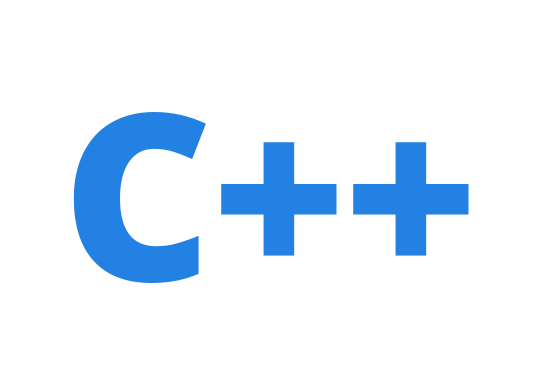
\includegraphics[width=0.6\linewidth]{CPP-Logo-Code}}
            \vspace*{3mm}
            \lstset{language=C++}
            \begin{lstlisting}
int sum(int *arr, int length) {
    int i, sum = 0;
    for(i = 0; i < length; i++) {
        sum += arr[i];
    }
    return sum;
}
            \end{lstlisting}
        \end{minipage}

        \vspace*{5mm}
        \noindent In the Haskell code, we define a function \textit{sum} using pattern matching. This function specifies that if it receives an empty list, the sum is 0. Otherwise, the list is divided into the first element \textit{x} and the rest of the list \textit{xs}. Recursion is then used to sum the remainder of the list until an empty list is encountered, at which point the recursion terminates.

        \newpage
        \subsection{Lazy Evaluation}

        \begin{minipage}[t]{0.45\textwidth}
            \raisebox{\depth}{
\includegraphics[width=\linewidth]{Haskell-Logo-Code}}
            \lstset{language=Haskell}
            \begin{lstlisting}
func arg =
  let x = func1 arg
      y = func2 arg
      z = func3 arg
  in if z then x else y
            \end{lstlisting}
        \end{minipage}
        \hfill
        \begin{minipage}[t]{0.45\textwidth}
            \centering
            \raisebox{-8mm}{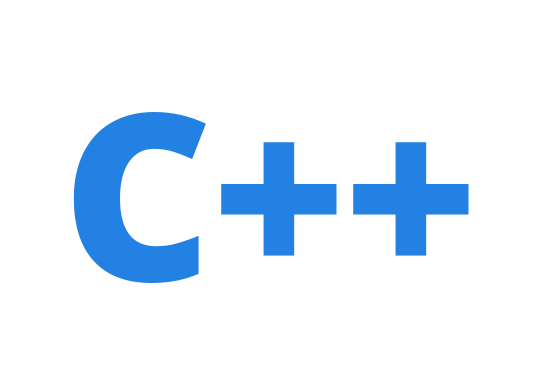
\includegraphics[width=0.6\linewidth]{CPP-Logo-Code}}
            \vspace*{3mm}
            \lstset{language=C++}
            \begin{lstlisting}
int func(int arg) {
    int x = func1(arg);
    int y = func2(arg);
    int z = func3(arg);
    if(z) {
        return x;
    } else {
        return y;
    }
}
            \end{lstlisting}
        \end{minipage}

    \vspace*{3mm}
    \noindent Let's assume \textit{func1}, \textit{func2}, and \textit{func3} each take 10 minutes to evaluate. In this C++ example, the code would approximately take 30 minutes to execute because C++ determines the values of \textit{func1}, \textit{func2}, and \textit{func3} sequentially. Conversely, Haskell employs lazy evaluation, only calculating these functions when necessary. In the given example, Haskell would first evaluate \textit{func3} (to determine \textit{z}), taking 10 minutes. Then, based on the value of \textit{z}, Haskell would evaluate either \textit{func1} or \textit{func2}—but not both. Thus, Haskell would require only 20 minutes in total to complete the execution.

    \newpage
    \subsection{Factorial}

    \begin{minipage}[t]{0.45\textwidth}
        \raisebox{\depth}{
\includegraphics[width=\linewidth]{Haskell-Logo-Code}}
        \lstset{language=Haskell}
        \begin{lstlisting}
factorial :: Integer -> Integer
factorial n
  | n <= 1    = 1
  | otherwise = n * factorial (n - 1)
        \end{lstlisting}
    \end{minipage}
    \hfill
    \begin{minipage}[t]{0.45\textwidth}
        \centering
        \raisebox{-8mm}{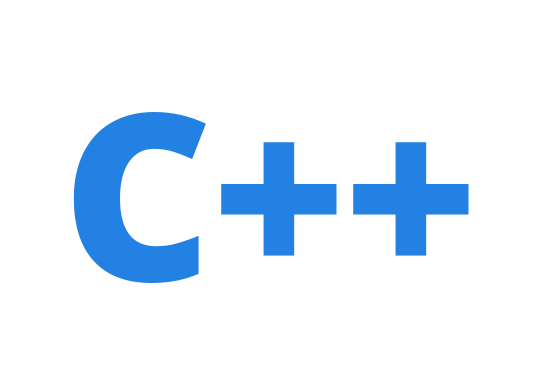
\includegraphics[width=0.6\linewidth]{CPP-Logo-Code}}
        \vspace*{3mm}
        \lstset{language=C++}
        \begin{lstlisting}
int factorial(int n) {
    if (n <= 1)
        return 1;
    else
        return n * factorial(n - 1);
}
        \end{lstlisting}
    \end{minipage}

    \vspace*{3mm}
    \noindent In both Haskell and C++, the factorial calculation is conceptually similar. Each language defines a function named \textit{factorial} that accepts an integer argument and returns an integer result. In Haskell, guard clauses are utilized to express that if \( n \leq 1 \), then the function should return 1; otherwise, it should return \( n \) multiplied by the factorial of \( n - 1 \), symbolized as \( n \times \text{factorial}(n - 1) \). This use of guard clauses is emblematic of Haskell's functional programming paradigm.

    \newpage
    \section{Conclusion}
    \noindent Throughout this document, we have examined Haskell, a language steeped in functional programming principles, and compared its features and structures with those of imperative languages such as C++. Through various examples, we have highlighted Haskell's strong static typing, lazy evaluation, and higher-order functions, which facilitate concise and expressive code. We observed the elegance of Haskell's pattern matching and the efficiency of its evaluation strategy, contrasting it with the explicit control flow and state management characteristic of C++.

    \noindent The comparison revealed the fundamental differences in approach between declarative and imperative programming. Haskell's guard clauses and recursive functions demonstrate its ability to abstract computations in a way that closely resembles mathematical definitions. Meanwhile, the C++ examples provided insight into the imperative paradigm's focus on step-by-step manipulation of program state.

    \noindent In practical terms, the choice between using Haskell or C++ can be influenced by several factors, including the nature of the problem, performance requirements, and the need for side-effect management. Haskell shines in domains where rigorous type safety and functional abstractions can lead to more reliable and maintainable code. On the other hand, C++ offers greater control over system resources and performance, making it suitable for applications where these are critical considerations.

    \noindent As programming paradigms continue to evolve, the insights gained from both Haskell and C++ will undoubtedly contribute to more robust and versatile software development practices. The strengths of Haskell's functional programming can inform and improve the design of software systems, even as we leverage the power and control offered by imperative languages like C++.

    \newpage
    \nocite{*}
    \printbibliography[heading=bibnumbered, title={References}]

	\section{Additional Resources}
	\section{Acknowledgments}
\end{document}
